Our test were performed mainly on two machines: one with an Intel® Core i7-7700 @ $3.6 \ GHz$ with $16 \ GB$ of RAM and one on an AMD® Ryzen 7 @ $3.6 \ GHz$ with $32 \ GB$ of RAM.
\subsection{PERM}
We want now to report an application of the PERM algorithm, made following the article's recipe \cite{PERM}.
The goal of this algorithm is to estimate the total number of fold and then simulate a finite number of SRCs hoping to find the energy minimum.
In the article the number of iterations is set to be $10^5$ for all proteins and the result is that they found only local minima, which are intermediate states.
We tried to improve these 2D simulations by increasing the number of iterations, hoping to find the real minimum reported in a well-known benchmark \cite{bench}.

The first protein for which we've improved the result is $HH(P)_5HH(P)_3H(P)_3HP$, that has a length of 18 amino acids (see Fig. \ref{fig:18_1}).
In particular, we've found $(1.25 \pm 0.35) \times 10^8$ folds with an energy minimum of -4 (a.u.), equal to the benchmark's one.
\begin{figure}[H]
    \centering
    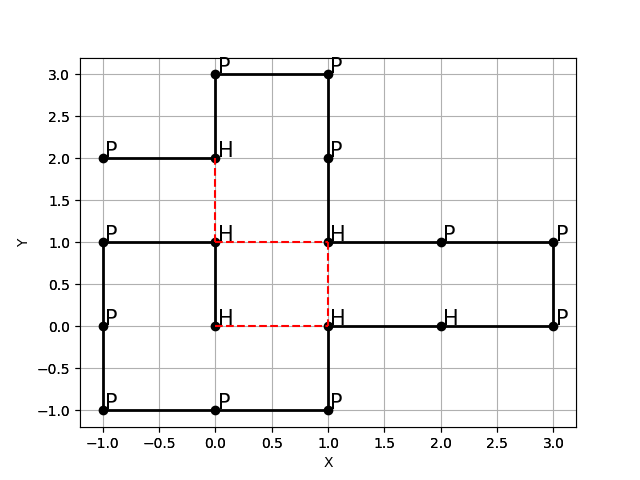
\includegraphics[width=.6\textwidth]{./img/18_1.png}
    \caption{\emph{The protein $HH(P)_5HH(P)_3H(P)_3HP$ has reached its energy minimum at -4 (a.u.) after $5 \times 10^6$ iterations ($\sim 20$ minutes).}}
    \label{fig:18_1}
\end{figure}
Another protein for which we've improved the result is $HHHP(PH)_3PP(HP)_3PH$, that has a length of 20 amino acids (see Fig. \ref{fig:20_2}).
In this case, we've found $(8.9688 \pm 0.0033) \times 10^{10}$ folds with an energy minimum of -9 (a.u.), one unit more than the benchmark's one.
\begin{figure}[H]
    \centering
    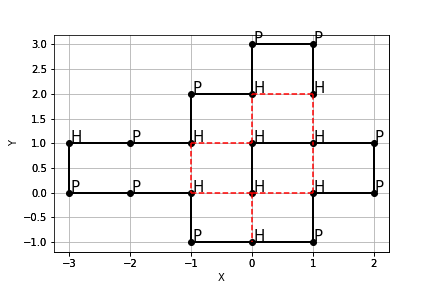
\includegraphics[width=.6\textwidth]{./img/20_2.png}
    \caption{\emph{The protein $HHHP(PH)_3PP(HP)_3PH$ has reached an energy minimum of -9 (a.u.) after $10^7$ iterations ($\sim 45$ minutes).}}
    \label{fig:20_2}
\end{figure}
We've also tried to improve the protein $HPHPHHH(P)_3HHHH(P)_2HH$, that has a length of 20 amino acids (see Fig. \ref{fig:18_2}).
However, after about 5 hours of running time it has folded with an energy of -7 (a.u.), like in the article, with an estimated number of folds equal to $(1.24 \pm 0.43) \times 10^8$.
\begin{figure}[H]
    \centering
    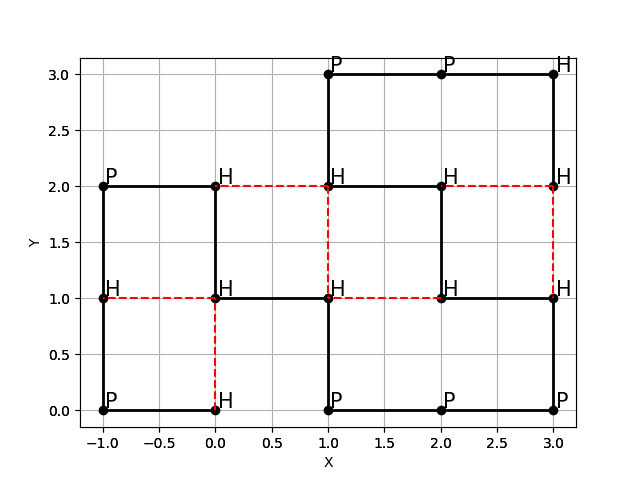
\includegraphics[width=.6\textwidth]{./img/18_2.png}
    \caption{\emph{The protein $HPHPHHH(P)_3HHHH(P)_2HH$ has reached an energy minimum of -7 (a.u.) after $10^8$ iterations ($\sim 5$ hours).}}
    \label{fig:18_2}
\end{figure}

\subsection{Constraint-based Protein Structure Prediction (CPSP)}
In the 2D case we showed that increasing the number of iterations resulted in better estimate of the energy.
However, the previous algorithm is not able to give significant outputs in the 3D case.
We tried so to estimate the energy in this case with another algorithm, which is based on constraint programming.
This is implemented by \emph{CPSP-tools} \cite{cpsp} and has revealed to be very powerful, folding proteins of length $\sim 200$ in few seconds.
Its velocity is based on an \emph{H-core database} that allows it to start from a known situation without going completely random.
Furthermore, this program is able to fold proteins in more complex lattices, like the 3D-face-centered-cubic one.
In our case, as we said, we wanted to improve the results of article \cite{PERM} so, in order to keep consistency, we opted for a 3D-cubic lattice.
All proteins tested converged to their energy minimum in less than a second, and we can see the results in Fig. \ref{fig:cpsp}.

\begin{figure}[H]
    \centering
    \begin{subfigure}[b]{0.45\textwidth}
        \centering
        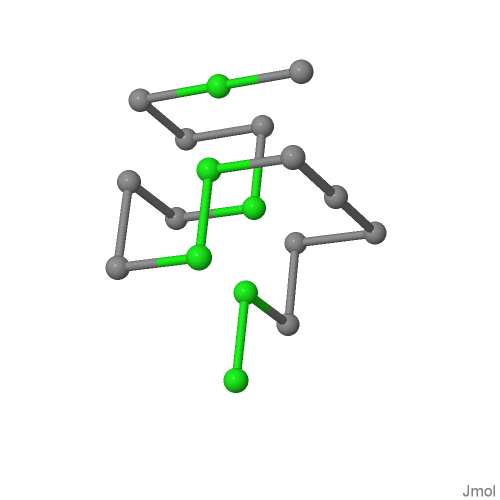
\includegraphics[width=\textwidth]{./img/18_3D.png}
        \caption{\emph{Energy $-4$ (a.u.) for the sequence $HH(P)_5HH(P)_3H(P)_3HP$.}}
    \end{subfigure}
    \begin{subfigure}[b]{0.45\textwidth}
        \centering
        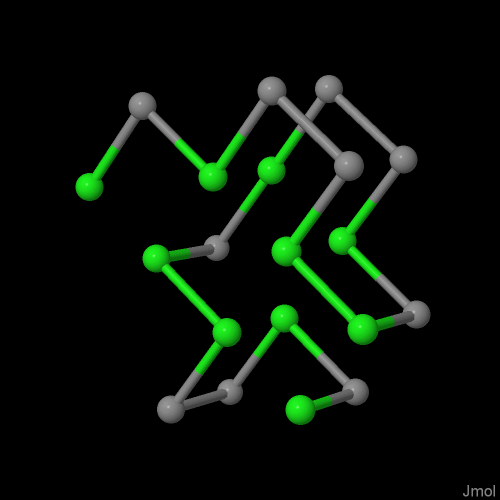
\includegraphics[width=\textwidth]{./img/20_3D.png}
        \caption{\emph{Energy $-11$ (a.u.) for the sequence $(HP)_2PH(HP)_2(PH)_2HP(PH)_2$.}}
    \end{subfigure}
    \begin{subfigure}[b]{0.45\textwidth}
        \centering
        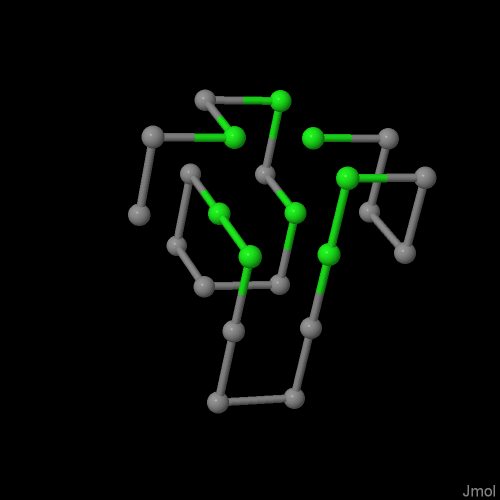
\includegraphics[width=\textwidth]{./img/24_3D.png}
        \caption{\emph{Energy $-8$ (a.u.) for the sequence $P(PH)_3(P)_4(HH(PP)_2)_2H$.}}
    \end{subfigure}
    \begin{subfigure}[b]{0.45\textwidth}
        \centering
        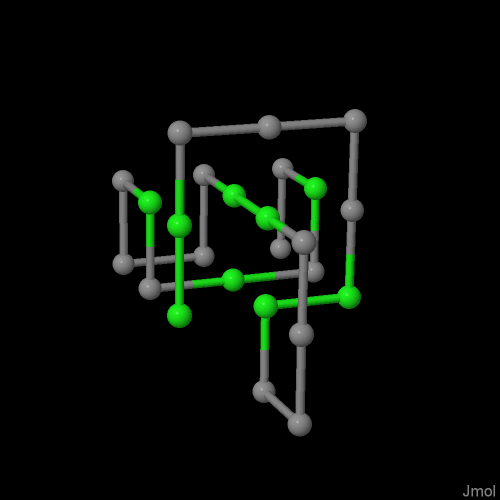
\includegraphics[width=\textwidth]{./img/25_3D.png}
        \caption{\emph{Energy $-8$ (a.u.) for the sequence $P(PH)_3(P)_4(HH(PP)_2)_2HH$.}}
    \end{subfigure}

    \caption{\emph{Four proteins of length 18 (a), 20 (b), 24 (c) and 25 (d).}}
    \label{fig:cpsp}
\end{figure}

\subsection{Reinforcement Learning}
Due to the fact that Reinforcement Learning code is extremely hard to write and optimize performance-wise, this section will only report in Tab. \ref{tab:RL} the main results obtained with DRL algorithms by \cite{jafari2020solving}.
These results are enough to show that DRL outperforms PERM and more in general brute force methods.

\FloatBarrier
\begin{table}[H]
\centering
\begin{tabular}[c]{ |p{8cm}||p{2cm}||p{2cm}|}
 \hline
 \multicolumn{3}{|c|}{Performance} \\
 \hline
 Sequence  & PERM & DRL\\
 \hline
$(HP)_2PH_2PHP_2HPH_2P_2HPH$ & $< 1$s & $< 1$s\\
 \hline
$P_2HP_2H_2P_4H_2P_4H_2P_4H_2$ & 6s  & $< 1$s\\
 \hline
$P_3H_2P_2H_2P_5H_7P_2H_2P_4H_2P_2HP_2$ & $< 1$s & $< 1$s\\
\hline
$P_2HP_2H_2P_2H_2P_5H_{10}P_6H_2P_2H_2P_2HP_2H_5$ & 3m & 25s\\
\hline
$H_2(PH)_3PH_4PHP_3HP_3HP_4$
$HP_3HP_3HPH_4(PH)_3PH_2$ & 3s & $< 1$s\\
\hline
$P_2H_3PH_8P_3H_{10}PHP_3H_{12}P_4H_6PH_2PHP$ & 7s & $< 1$s\\
\hline 
$H_{12}(PH)_2(P_2H_2)_2P_2H(P_2H_2)_2P_2HPHPH_{12}$ & 78h & 48m\\
\hline
$H_4P_4H_{12}P_6(H_{12}P_3)_3HP_2(H_2P_2)_2HPH$ & 64s & 1s\\
\hline
$P_3H_2P_2H_4P_2H_3(PH_2)_3H_2P_8H_6P_2H_6P_9$
$HPH_2PH_{11}P_2H_3PH_2PHP_2HPH_3P_6H_3$ & 1h & 4m\\
\hline
$P_6HPH_2P_5H_3PH_5PH_2(P_2H_2)_2PH_5PH_{10}$
$PH_2PH_7P_{11}H_7P_2HPH_3P_6HPHP_2$ & 9m & 1m\\
\hline

\end{tabular}\\
\caption{\emph{Performance of Perm and Deep Reinforced Learning on the same protein sequence, the energy was omitted because for each sequence both model found the same energy of the folded state.}}
\label{tab:RL}
\end{table}

\FloatBarrier

